%--------------------------------------%
\chapter{Language Server Architecture}
%--------------------------------------%

\begin{chapterabstract}
	\dots in which we introduce language servers in general and the
	\acrlong{lsp} in particular, outline their relationship to other classes of
	language tooling, and look at high-level architectural decisions that their
	use-cases imply.
\end{chapterabstract}

Language servers have a lot in common with compilers. Like compilers, they have
to build up a semantic model of a program and provide useful diagnostics for
invalid or suspicious input along the way. Unlike a compiler, a language server
needs to maintain the semantic model over the course of an editing session.
Rather than operating in batch mode, a language server runs continuously and is
expected to provide feedback within milliseconds.

However, language servers need neither to produce compilation artifacts nor to
optimise the programs they process. Instead, they are effectively
special-purpose query engines. Their output is a data structure optimised for
fast querying, such as finding references, definitions, or providing
context-sensitive completion suggestions. From that point of view, it could seem
like a language server is merely a compiler frontend with very little backend
logic. Unfortunately, this is not the case.

The requirement for real-time feedback to the developer is the primary
constraint on a language server's design. For all but the most basic languages
and features, instant feedback requires an incremental computation approach and
management of state that persists across updates to source files. The second
most important consideration, and one to a large extent not shared with
compilers, is resilience to errors. While a compiler generally expects
well-formed input, a language server deals with all sorts of intermediate states
of a document, including files with many syntactic errors, invalid encodings, or
unsaved buffers outside the filesystem.

To make matters worse, while compiler frontend implementations are often guided
by a language specification\footnote{Even if, usually, an informal one.}, the
space of invalid programs is unconstrained. Developers of language servers have
to guess what intermediate states a program goes through during development and
how to respond to them. Generating meaningful semantic models from invalid input
is a challenging task, but doing so is often crucial for developers. For
example, smart auto-completion in statically typed languages is expected to
provide type-correct suggestions, even as the document being edited is
type-incorrect, and often semantically or even syntactically invalid.

In this chapter, we explore the status quo of language servers, how they differ
from conventional batch-processing compilers, how this gap may narrow in the
future, and what makes building interactive language tooling difficult.

%----------------------------------------%
\section{The fruits of semantic support}
%----------------------------------------%

\todo[inline]{
	should cover LSP ``language features'' section, current tooling, show
	especially limitations of current tools with invalid input, guessing,
	complex situations (rust-analyzer failing to infer types rustc knows about),
	etc
}

The largest language servers conforming to \acrshort{lsp} offer a wide variety
of features. The vast majority of the \acrshort{api} surface is optional,
however. Upon establishing a connection, the client and server exchange
information about their respective capabilities, establishing a subset of
\acrshort{lsp} they both support.

The functionality of \acrshort{lsp} comes in two main flavours: code
comprehension and coding features. The former subsumes utilities which ease
reading and navigating through code, such as Hover (where the editor displays
details about an object under the pointer), Go to Definition, Find References,
etc. Utilities like diagnostics, auto-completion, or code actions are more
relevant to the programmer at the time they are authoring code and belong in the
latter category.

Next, we will delve into both categories and take a closer look at what they
offer.


\subsection{Code comprehension in \pdfacrshort{lsp}}

\todo[inline]{this is lsp 3.17}

\newcommand{\org}{\pdftooltip{(original)}{This request was present in the
original LSP specification.}}

Code comprehension functionality takes up the majority of \acrshort{lsp}'s
\acrshort{api} surface and has been growing during the protocol's evolution. The
central features, already present in the initial specification of the protocol,
are Go to Definition, Find References, Document Highlight, Document Link, Hover,
Code Lens, and Document Symbols\todo{examples for everything, including a
screenshot from Neovim or something that's not VS Code. Don't forget to add
Haskell evaluation code lenses.}.

\begin{figure}[h]
	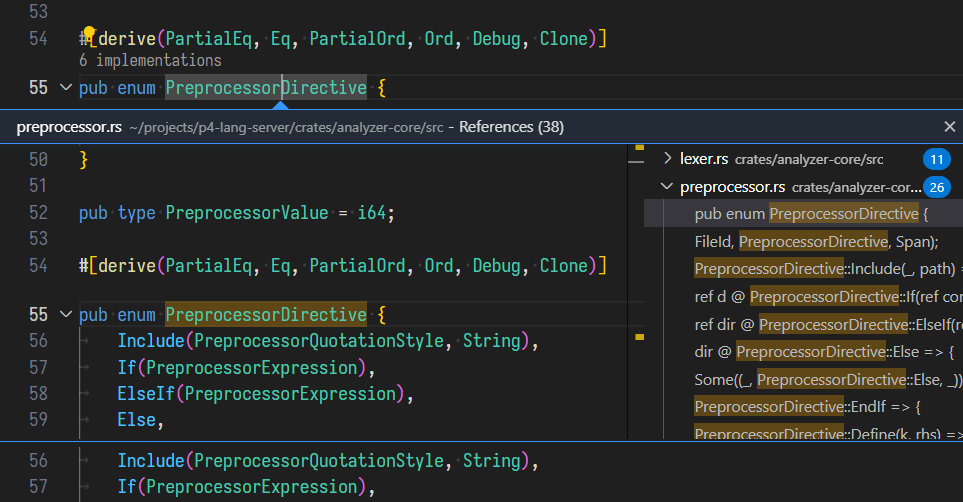
\includegraphics[width=1.00\textwidth]{resources/code_find_references.png}
	\caption{Find References in Visual Studio Code via rust-analyzer.}
\end{figure}

Go to Definition and Find References are
present in some of the oldest code comprehension tools, dating back at least to
the Unix utility \texttt{ctags}\cite{exuberant-ctags}. These let the editor jump
from a symbol's use-site to its definition and vice versa, just as their names
imply. \acrshort{lsp}'s Document Highlight request does not provide syntax
highlighting, rather, it serves to visually assist the programmer with locating
references of a given symbol without having to explicitly invoke the Find
References feature. Document Highlight could be merged with Find References
functionality, but the \acrshort{lsp} maintainers choose to keep them separate
and allow Document Highlight to report imprecise (``fuzzy'') matches. A response
to the Document Link request lists the hyperlinks embedded in the document.
Document Symbols provides a potentially hierarchical overview of the symbols of
a document, which serves the ``outline'' feature of modern editors: a tree
overview of a program's constructs, such as modules, classes, fields, and
methods. The Hover feature provides additional contextual information when
navigating code. It is typically implemented by the client rendering a pop-up
box of documentation for a given symbol. Finally, Code Lens is a versatile
editor feature for displaying additional information at a given position in a
document, such as the number of references of a type or the code metrics of a
procedure\cite{codelens-comparison}. It can trigger an action when activated,
which is used by some servers to run tests or open a Find References dialog.

\begin{figure}[t]\centering
	\begin{multicols}{2}
	\begin{enumerate}
		\item Go to Declaration
		\item Go to Definition \org
		\item Go to Type Definition
		\item Go to Implementation
		\item Find References \org
		\item Prepare Call Hierarchy
		\item Call Hierarchy Incoming Calls
		\item Call Hierarchy Outgoing Calls
		\item Prepare Type Hierarchy
		\item Type Hierarchy Super Types
		\item Type Hierarchy Sub Types
		\item Document Highlight \org
		\item Document Link \org
		\item Document Link Resolve \org
		\item Hover \org
		\item Code Lens \org
		\item Code Lens Refresh
		\item Folding Range
		\item Selection Range
		\item Document Symbols \org
		\item Semantic Tokens
		\item Inlay Hint
		\item Inlay Hint Resolve
		\item Inlay Hint Refresh
		\item Document Color
	\end{enumerate}
	\end{multicols}

	\caption{Code comprehension -related requests in \acrshort{lsp} 3.17.}
	\label{fig:comprehension-requests}
\end{figure}


\subsection{Coding features in \pdfacrshort{lsp}}

A shorter but no less important range of \acrshort{api} calls supports the
developer right when they are authoring code. The main features are
auto-completion, signature help, formatting, and symbol renaming.

\begin{figure}
	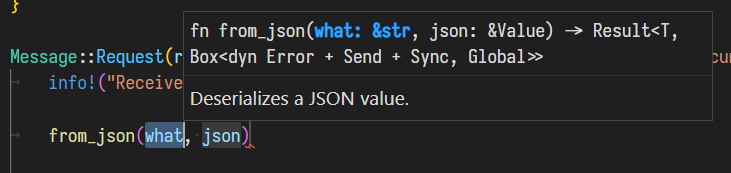
\includegraphics[width=1.00\textwidth]{resources/code_signature_help.png}
	\caption{Signature help in VS Code for Rust shows a pop-up with
	documentation as well as the signature of the callee, highlighting the
	parameter under cursor.}
\end{figure}

Auto-completion offers to fill in code as the programmer is typing, supports
ranking results based on their relevance, on both the server and the client
side, and can include a ``quick info'' description for each option. Signature
help shows parameter name and type information when calling a procedure, method,
or function. Formatting allows a language server to rewrite a document upon
request, for example to conform to a particular code style. The \acrshort{lsp}
formatting functionality can format either the entire document, a selected
range, or reactively an arbitrary part of the document as the user types.
Finally, symbol renaming performs a context-sensitive workspace-wide rename of a
given symbol.

\begin{figure}[t]\centering
	\begin{multicols}{3}
	\begin{enumerate}
		\item Inline Value
		\item Inline Value Refresh
		\item Moniker
		\item Completion Proposals \org
		\item Completion Item Resolve \org
		\item Publish Diagnostics
		\item Pull Diagnostics
		\item Signature Help \org
		\item Code Action
		\item Code Action Resolve
		\item Color Presentation
		\item Formatting \org
		\item Range Formatting \org
		\item On type Formatting \org
		\item Rename \org
		\item Prepare Rename
		\item Linked Editing Range
	\end{enumerate}
	\end{multicols}

	\caption{Coding language features in \acrshort{lsp} 3.17.}
	\label{fig:coding-requests}
\end{figure}

Later \acrshort{lsp} revisions added high-level features not universally
applicable to all programming languages. For instance, version 3.16 added
\emph{linked editing}, which some conforming implementations use to update
opening and closing \acrshort{xml} tags seamlessly without the user specifically
triggering a rename action. Version 3.17 introduced \emph{type hierarchy}
requests, relevant only to programming languages with subtyping. On the other
hand, more general facets of the protocol see creative use in unintended
contexts. One example is the use of lenses and special comments in the Haskell
Language Server project\cite{haskell-ls} to provide \acrshort{repl}-like
functionality. Another is the LT$_\text{E}$X Visual Studio Code
extension\cite{vscode-spellcheck}, which provides spell and grammar checking in
Markdown and \LaTeX{} documents, as well as in programming language comments.
Even though \acrshort{lsp} has no built-in support for extracting the comments
of a document or for spell checking in general, LT$_\text{E}$X achieves this
with a combination of non-\acrshort{lsp} \acrshort{api}s and by leveraging
\acrshort{lsp} diagnostics and code actions to provide suggested spellings.

\begin{figure}[h]\centering
	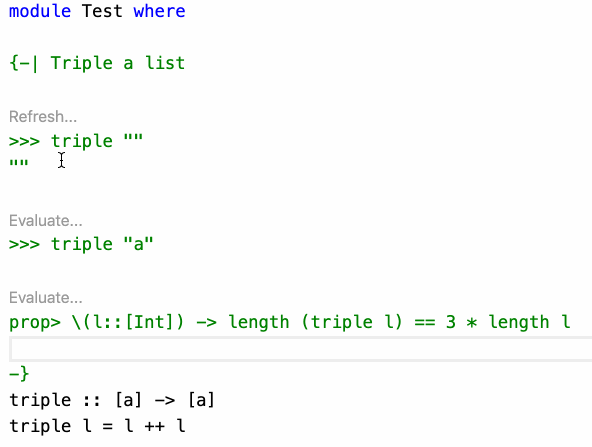
\includegraphics[height=0.3\textheight]{resources/code_haskell_repl.png}
	\caption{The Haskell Language Server project supports in-editor expression
	evaluation in comments prefixed with \texttt{>>>} and checking QuickCheck
	properties in comments starting with \texttt{prop>}.}
\end{figure}

\subsection{The state of the art}

Some of the best tooling in the \acrshort{lsp} ecosystem comes, somewhat
unsurprisingly, from Microsoft.

Projects which served as the de facto \acrshort{ide} integration for the given
language matured somewhat quicker than software that already had ample
competition.

\todo[inline]{the idea here is to compare "actual" language popularity
with the popularity of a corresponding language server.
We should see people preferring other tools for established technologies.}

We have chosen to exclude some technologies from this comparison. JavaScript,
TypeScript, CSS, and HTML support is built into VS Code and therefore does not
show up in VS Code marketplace statistics for installed language extensions.
SQL, while popular, has too many dialects to present a faithful picture through
the lens of extension installations alone. These technologies were in turn
filtered out from StackOverflow's list of most popular languages to highlight
the differences in ranking.

\todo[inline]{
	add the source
	% https://marketplace.visualstudio.com/search?target=VSCode&category=Programming%20Languages&sortBy=Installs
}

\begin{table}\centering
\caption{Popularity of programming languages among VS Code users and
StackOverflow's 2022 Developer survey\cite{stackoverflow-survey-2022}
respondents.}
\begin{tabular}{|r|c|c|}
	Rank & VS Code extension & Most popular programming and scripting languages
	\tabularnewline \hline
	1  & Python     & Python     \tabularnewline
	2  & C/C++      & Java       \tabularnewline
	3  & Java       & C\#        \tabularnewline
	4  & C\#        & C/C++      \tabularnewline
	5  & Go         & PHP        \tabularnewline
	6  & PHP        & PowerShell \tabularnewline
	7  & PowerShell & Go         \tabularnewline
	8  & Dart       & Rust       \tabularnewline
	9  & Ruby       & Dart       \tabularnewline
	10 & Rust       & Ruby       \tabularnewline
\end{tabular}
\end{table}

\todo[inline]{the whole thing above is kinda suspicious.
I'm not sure a comparison like that has a place in a language server thesis.}

%----------------------------------------%
\section{Lessons from the compiler world}
%----------------------------------------%

We have previously established how closely does the task of implementing
language servers relate to writing compilers. Let us expand on the possible
architectural similarities of the two kinds of language tools in this section.

\subsection{The pipeline}

Traditional compiler architectures build around a pipeline approach. The
compiler begins with a frontend, typically composed of a lexer\footnote{Although
the lexer/parser distinction is maintained, partly for historical reasons, in
many modern compilers, the jobs of lexers and parsers are conceptually
identical. These compositional algorithms transform input of one type (usually a
string) into output of another, verifying certain properties along the way.
Concretely, they match the input against some
grammar\footnotemark.}\footnotetext{A keen reader will note that without
restrictions on the \emph{class} of grammars, this statement makes the
description no more concrete.}, a parser, and a step of semantic analysis. The
second major part is the backend, a combination of an optimiser and a code
generator. The lexer ingests bytes of text, turning them into tokens for the
parser. The parser matches the tokens against the productions of a given
language's grammar, producing \acrlong{ast}s. Semantic analysis then verifies
that the parsed program adheres to the language's semantic restrictions. For
example, semantic analysis ensures that variables can only be referenced after
their declaration or definition, \texttt{break} statements can only appear in
the bodies of loops, and the program follows typing rules.

Is it the frontend's responsibility to identify and report user errors,
terminating the compiler pipeline as soon as it identifies invalid input. This
is a practical choice, since later stages of the compiler can assume the program
valid and not worry about possible errors. Furthermore, computation of the
backend stages would be wasted on invalid input anyway, as the compiler could
give no guarantees about the produced executable form\footnote{Whether that is
machine code in a platform-specific executable, bytecode for a virtual machine,
source code in the case of transpilers, or something else entirely.}.

One important step that typically happens on the frontend/backend boundary is
\emph{lowering}. This process turns the \acrshort{ast} obtained and validated by
previous stages into the compiler's \emph{\acrfull{ir}}. The \acrshort{ir}
represents a simplified language devoid of syntactical sugar and various
programmer-facing niceties. For example, various types of conditional
expressions are usually represented by a single \acrshort{ir}
instruction\footnote{Which may in fact conceptually be an instruction, or a node
of the \acrshort{ir} graph.}. Similarly, different forms of loops lower to a few
canonical translations. Freedoms in the source-level code style are eliminated
to make reasoning about the program further down the pipeline easier. Nested
expressions are flattened using short-lived local variables, often imposing an
evaluation order. Overall, \acrlong{ir}s tend to be semantically closer to the
target architecture.

After lowering, the backend takes over. The optimizer, if it is involved in the
compilation, iteratively transforms the \acrshort{ir} in a series of analysis
and rewriting steps that attempt to minimise certain cost functions\footnote{The
actual cost functions may vary based on what steps the optimizer takes. For
example, the metrics used for inlining can differ from heuristics consulted for
loop-invariant code motion.}. Optimization can sometimes cross the boundaries of
source-level code. That is, certain \acrshort{ir} programs do not have a
corresponding source program, because the lowering phase is not a surjective
mapping. This is a necessary freedom for eliminating overhead in implementations
of high-level programming languages, but makes mapping issues in the final
executable more difficult\footnote{Which is of major concern for debugging, and
consequently one of the primary reasons why native executable debuggers tend to
operate better on programs compiled with fewer optimizations.}.

Finally, the pipeline terminates in a code generation phase which emits the
final executable form. This step requires rewriting the \acrshort{ir} program in
order to fit the target constraints. The amount of work the compiler needs to do
in this last stage depends on the semantic differences between the structure of
the \acrlong{ir} and the target language. It could be as simple as writing the
\acrshort{ir} to an output file, if the intermediate and target languages
perfectly match. For conventional processor targets, however, code generation
necessitates at least instruction selection and register allocation, as well as
maintaining some level of conformance to standard calling conventions.

\subsubsection*{Born of necessity, sculpted for collaboration}

\todo[inline]{Figure out where did the pipeline design come from, how GCC
popularised it (I swear I heard that somewhere)}

\subsubsection*{Where the pipeline falls short}

In recent years, the feedback loop from writing code to executing it has gotten
shorter and shorter. The case for early feedback is simple: programmers want
results as soon as possible. Moreover, since the programmer typically uses the
compiler in an online fashion, changes to the source files tend to be small and
local. Compiling small changes in the source program often only requires small
changes to the output. With proper caching, most information can be reused from
previous runs of the compiler.

With semantic language support receiving more and more attention, the overlap
between compilers and interactive language tooling is only getting clearer. Both
classes of programs now need to maintain and incrementally update databases of
semantic information about the codebase in order to respond quickly to user
requests. With semantic information at hand, it is only natural for both classes
to integrate tightly with editors and development environments to provide
features reliant on high-level information. Both compilers and language servers
should be resilient to errors in the user input and continue processing as far
as is practical, for example to report semantic errors even in the presence of
syntactical issues. Just as with optimizers\todo{make sure we reference the
previous subsubsection here correctly}, reimplementing a lot of complicated
functionality is tiresome and unnecessary.

Unfortunately, the well-established pipeline approach to compiler construction
is, despite its many innovations, difficult to adapt to the modern incremental
workloads. The interfaces between stages do not share a principled, universal
structure, requiring each phase to implement its own variant of caching and
cache-invalidation. Running phases concurrently for independent sections of the
input program can be problematic, because older pipeline-based compilers often
rely on global variables\footnote{This is no fault of the architecture as a
whole, but it is an important practical consideration.}.

Conventional incremental compilers choose a granularity of input file,
compilation unit, or module, and often run several pipelines in parallel,
culminating in a sequential step that combines the constituent products into the
final executable. This approach achieves very short compilation and
recompilation times for many programs, but tends to produce suboptimal code,
since the optimiser can only see a subset of the code and is limited in
attempting whole-program optimisation and cross-module inlining. Nowadays,
linkers (the usual last step in the production of executables) counter this
downside with \acrfull{lto}, trading linking time for better quality code.
Running many pipelines in parallel also tends to increase the size of the
intermediate compilation artifacts, because dead code elimination cannot safely
remove unused definitions, possibly referenced by other compilation units.

\subsection{The pipeline as a sequence of queries}

With these new developments and performance constraints in mind, recent compiler
construction techniques put incremental computation at the centre of their
design. For example, Roslyn\footnote{This product is officially called \emph{The
.NET Compiler Platform SDK} but it is arguably better known under the Roslyn
codename.}, a collection of compilers and analysers for C\# and Visual Basic,
builds heavily on incremental computation. A Roslyn compiler takes centre stage
in a number of interactive and batch applications, maintaining a semantic model
of the codebase. Higher-level tools then query and update this model via several
\acrshort{api}s designed for static analysis, code refactoring, and other
use-cases\cite{roslyn-apis}\todo{what are some concrete applications that build
on these?}. The entire stack is optimised for interactive use. For example, the
parsers utilise a combination of persistent ``green'' \acrlong{ast}s and
transient ``red'' trees. The second, ephemeral type is built on-demand,
optimised for querying, and discarded with edits\cite{roslyn-red-green-trees},
while the ``green'' tree serves as the source of truth.

As more and more language tools interact with and rely on the compiler, compiler
authors find themselves adapting the pipelined architecture to emit additional
intermediate artifacts. If this evolution happens organically over long periods
of time and without a methodical approach, compiler codebases can degenerate
into clouds of complex, intertwined code.

A possible remedy is to adapt the pipeline architecture in ways that make it
simple to incrementalise and memoize its stages. The key insight is that the
pipeline is conceptually a collection of data-dependent queries. If we express
the compiler in the language of a general query engine, caching and incremental
computation features come for free. Propagating changes through the data
dependency graph is simple, and this change processing subsumes cache
invalidation. The interfaces between compiler queries effectively become
high-level \acrshort{api}s, with little extra work. These interfaces are shared
with other applications, making integration simpler and less error-prone than in
many traditional pipeline architectures, which maintain separate sets of
internal and external interfaces.

\subsubsection*{A functional approach}

Even though the traditional pipeline and its query-based reimagination are
conceptually close, their implementations are vastly different. Typical
compilers mutate global state during the course of a compilation. If any stages
produce additional data, they populate side channels in the form of global maps
and tables for further passes to use. This can lead to subtle compiler bugs when
compiler passes are added, removed, or reordered. Mutable state is also an
obstacle to parallelism and makes it difficult to reason about where exactly in
the pipeline does one intermediate form change into another.

On the other hand, the query-based approach is inherently functional. Compiler
passes are ordered by their data dependencies and the amount of available
parallelism is limited only by the number of independent queries at a given
stage. A query-based compiler should avoid using mutable state, so that the
query engine can correctly propagate changes and update memoized
functions\footnote{Some hidden mutability may still be beneficial for
performance optimisations. For example, a hidden mutable map can serve as a
backing store for string interning. Naturally, the programmer needs to be
vigilant around any such places in the implementation and verify that the
introduced side-effects do not compromise correctness of the entire system.}.

\subsubsection*{Queries in the wild}

The Rust compiler was not originally built around a query system, but one has
been retrofitted into it, and major parts of the pipeline between
\texttt{rustc}'s high-level \acrshort{ir} and \acrshort{llvm} \acrshort{ir} are
now implemented as incremental interdependent queries.\todo{reference}

The Roslyn project\todo{add information from the GitHub discussions thread, once
available.}

\todo[inline]{include citations of the Sixten compiler, the rock library that
supports Sixten, the talk by Anders, and \texttt{rustc} queries. Also, build
systems a la carte, perhaps?}
